\begin{figure}[t!]
    \centering
    \begin{subfigure}[b]{\textwidth}
        \centering




















        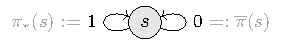
\includegraphics[width=0.35\linewidth]{figures/mdp.pdf}
        \caption{MDP}
        \label{fig: experiment smallest MDP for iv vs fv}
    \end{subfigure}%
    \\
    \vspace{0.5cm}

    \begin{subfigure}[b]{0.48\textwidth}



















                







                


                

                



                




        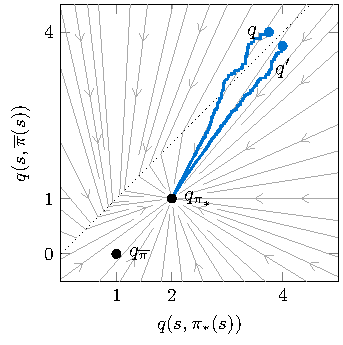
\includegraphics[width=0.8\linewidth]{figures/iv-sol.pdf}
        \caption{Initial-visit solutions}
        \label{fig: iv versus fv simulations IV}
    \end{subfigure}
    \hfill

    \begin{subfigure}[b]{0.48\textwidth}



















                







                


                

                



                




        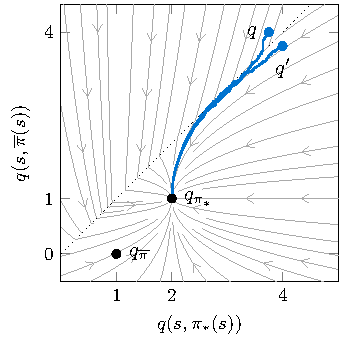
\includegraphics[width=0.8\linewidth]{figures/fv-sol.pdf}
        \caption{First-visit solutions}
        \label{fig: iv versus fv simulations FV}
    \end{subfigure}
    \caption{By avoiding sliding modes, initial-visit solutions sometimes converge to the optimal policy $\best{\pi}$ faster than first-visit solutions despite fewer updates and smaller effective learning rates. The blue lines are MC-O-PI solutions starting in $q$ or $q'$, whereas the grey lines indicate the mean-field flow.}
    \label{fig: iv versus fv simulations}
\end{figure}
